\section{Ejercicio 4}
\noindent
En la siguiente secci\'on se busca analizar los tiempos caracter\'isticos de la compuerta 74HC02, medidas con carga y sin carga. Adem\'as se analizar\'a la respuesta de la fuente de alimentaci\'on de las compuertas, trabajando en altas frecuencias.
\subsection{Desarrollo emp\'irico}
\noindent
Inicialmente se midi\'o la salida de la compuerta NOR, de tecnolog\'ia CMOS, con las entradas cortocircuitadas y sin carga, y luego con el circuito propuesto en la figura \ref{ej4_fig:circuito}, buscando medir el \textit{time rise}, el \textit{fall time} y el tiempo de propagaci\'on en la transici\'on del estado alto a bajo, y del estado bajo al alto.\\
\begin{figure}[H]
    \centering
    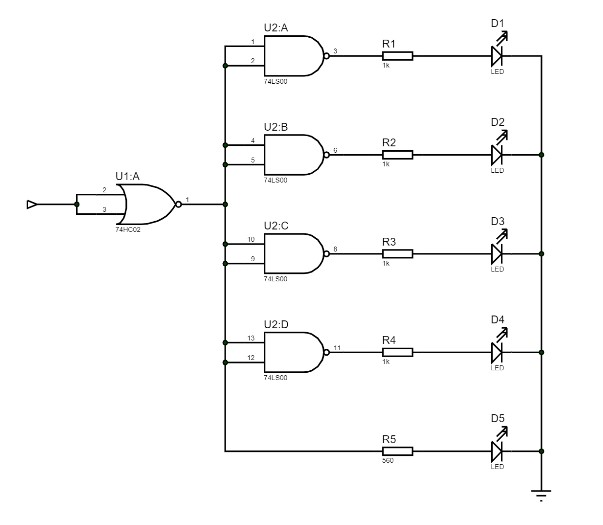
\includegraphics[width=0.5\linewidth]{figs/EJ4/esquematico.jpg}
    \caption{Circuito de medici\'on}
    \label{ej4_fig:circuito}
\end{figure}
Para los cuatro tiempos a medir se utilizaron los cursores del osciloscopio utilizando la funci\'on de \textit{tracking} como se ejemplifica en la figura \ref{ej4_fig:HC}.
\begin{figure}[H]
\begin{subfigure}{.5\textwidth}
  \centering
  % include first image
  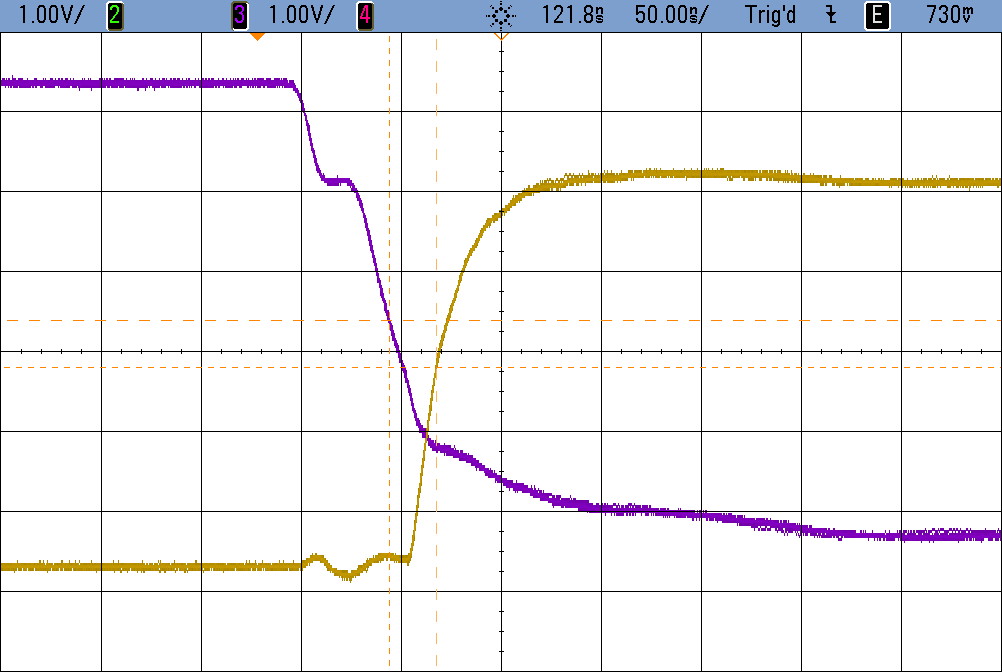
\includegraphics[width=.85\linewidth]{figs/EJ4/HC_Prop.png}  
  \caption{Medici\'on del tiempo de propagaci\'on.}
  \label{ej4_fig:HC_prop}
\end{subfigure}
\begin{subfigure}{.5\textwidth}
  \centering
  % include second image
  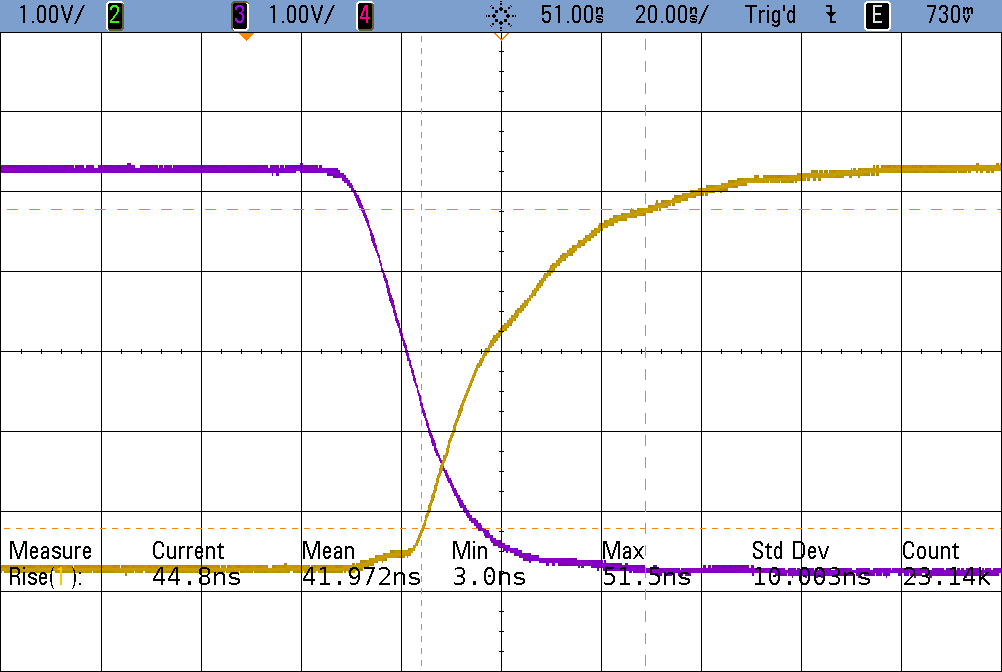
\includegraphics[width=.85\linewidth]{figs/EJ4/HC_TR.png}  
  \caption{Medici\'on del \textit{time rise}.}
  \label{ej4_fig:HC_rise}
\end{subfigure}
\caption{Mediciones sobre la compuerta, violeta-entrada, amarilla-salida}
\label{ej4_fig:HC}
\end{figure}
De estas mediciones se obtuvieron los resultados de la tabla \ref{ej4:table_times}, en todos los casos se puede apreciar que los tiempos con carga son mayores que sin carga, sin embargo dichas asimetr\'ias son despreciables y las mismas pueden ser explicadas debido a la demanda de corriente de la rama de $R_5$ y $D_5$. 
\begin{table}[H]
\centering
\begin{tabular}{|c||c|c|}
\hline
          & Sin carga & Con carga \\ \hline \hline
$t_r$     & 43       & 45       \\
$t_f$     & 44,5     & 48       \\
$t_{prop H-L}$ & 10,5     & 12      \\
$t_{prop L-H}$ & 13,5     & 15,5     \\ \hline
\end{tabular}
\caption{Mediciones de tiempos caracter\'isticos, en ns.}
\label{ej4:table_times}
\end{table}
\subsection{Medici\'on a altas frecuencias}
\noindent
Una vez medidos los tiempos caracter\'isticos, para continuar el an\'alisis se aumento la frecuencia del generador a 100KHz, y se midi\'o la alimentaci\'on de la compuerta 74HC02.\\
\begin{figure}[H]
\begin{subfigure}{.5\textwidth}
  \centering
  % include first image
  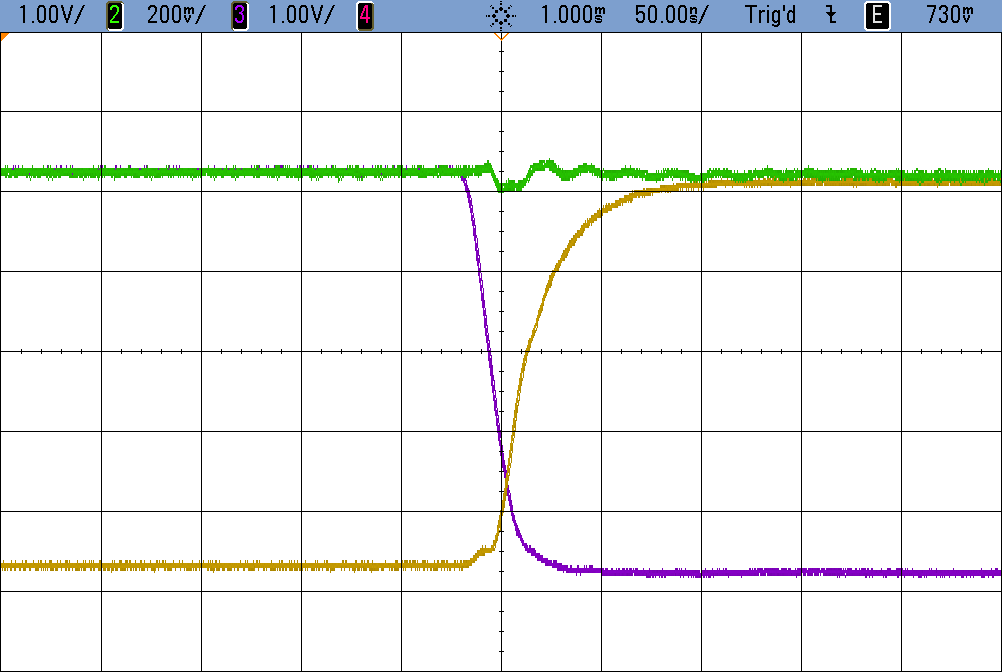
\includegraphics[width=.85\linewidth]{figs/EJ4/HF_sin_C.png}  
  \caption{Sin capacitor de desacople.}
  \label{ej4_fig:HF_sin_C}
\end{subfigure}
\begin{subfigure}{.5\textwidth}
  \centering
  % include second image
  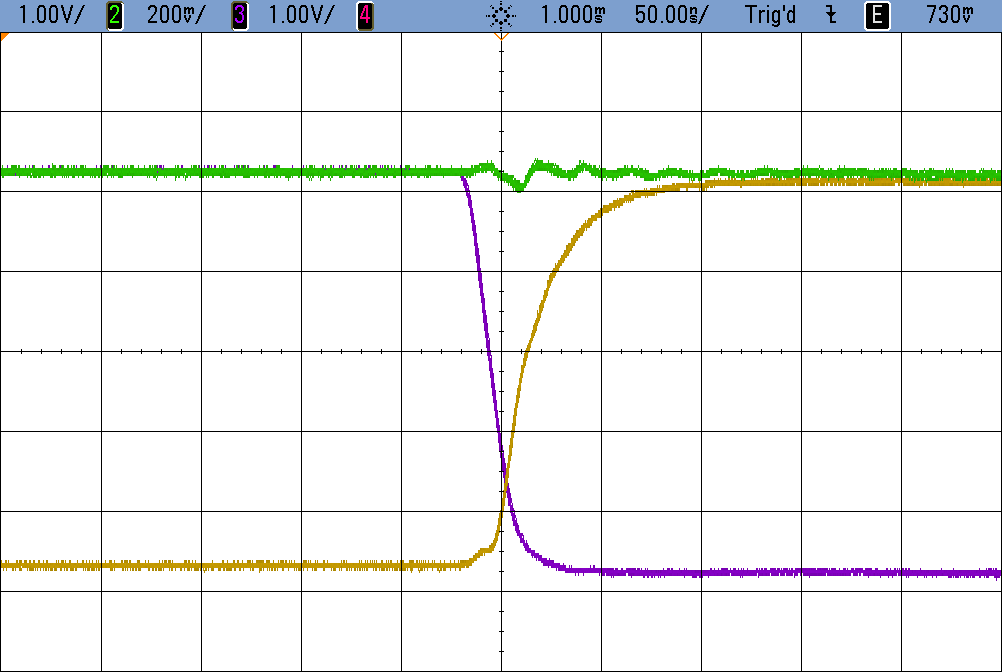
\includegraphics[width=.85\linewidth]{figs/EJ4/HF_con_C.png}  
  \caption{Con capacitor de desacople.}
  \label{ej4_fig:HF_con_C}
\end{subfigure}
\caption{Medici\'on de la alimentaci\'on (verde), salida (amarilla), entrada (violeta)}
\label{ej4_fig:HF}
\end{figure}
En la figura \ref{ej4_fig:HF_sin_C}, se puede apreciar que en la transici\'on de estados, en la alimetaci\'on se produce una respuesta subamortiguada, esto es debido a una mayor exigencia de corriente en dicho momento por parte del integrado.\\
Se intent\'o cambiar dicha respuesta con la inclusi\'on de un capacitor de desacople en los terminales de alimentaci\'on del integrado, el mismo seg\'un lo especificado en el libro de aplicac\'on  del fabricante\footnote{http://www.ti.com/lit/an/sdya002/sdya002.pdf} debe ser de 100nF. Agregando dicho capacitor al circuito se busc\'o reducir dicha respuesta subamortiguada, lo obtenido se muestra en la figura \ref{ej4_fig:HF_con_C}, en la que es posible observar que no se logr\'o corregir completamente el comportamiento indeseado de la fuente, sin embargo se redujo su duraci\'on levemente.\\
Al trabajarse con una sola de las compuertas las demandas de corriente al circuito de alimentaci\'on no fueron excesivas, pero si se hubiese trabajado con la totalidad de las compuertas integradas, el capacitor de desacople hubiese cumplido una funci\'on de mayor relevancia.
\subsection{Conclusiones}
\noindent
Midiendo los tiempos caracter\'isticos de la compuerta 74HC02 de tecnolog\'ia CMOS se pudo observar la influencia de la carga en los mismos, viendo que al aumentar los niveles de carga, aumentaban tanto el tiempo de propagaci\'on como el \textit{rise time} y el \textit{fall time}.\\
Adicionalmente fue posible observar que dependiendo las condiciones de trabajo puede ser necesaria la inclusi\'on de capacitores de desacople al utilizar integrados l\'ogicos, ya que la respuesta transitoria de la fuente de alimentaci\'on puede generar niveles de tensi\'on que se encuentren fuera del rango permitido por el fabricante. 